%%%%%%%%%%%%%%%%%%%%%%%%%%%%%%%%%%%%%%%%%%%%%%%%%%%%%%%%%%%%%%%%%%%%%%%%%%%%%%%%
\exercice{Réduction de schéma-bloc~\moyen}
%%%%%%%%%%%%%%%%%%%%%%%%%%%%%%%%%%%%%%%%%%%%%%%%%%%%%%%%%%%%%%%%%%%%%%%%%%%%%%%%

\question{}
Le schéma-bloc dans le cas pour lequel l'entrée $P$ est nulle est donné 
ci-dessous
%-------------------------------------------------------------------------------
\begin{center}
    \tikzsetnextfilename{ex1-q1-chap_bloc-ext}
    \input{tikz/ex1-q1-chap_bloc.tex}
\end{center}
%-------------------------------------------------------------------------------

\question{}
Pour déterminer la fonction de transfert $H_E(p)$, il nous faut réduire le
schéma-bloc précédent.
%-------------------------------------------------------------------------------
\begin{center}
    \tikzsetnextfilename{ex1-q2-chap_bloc-ext}
    \input{tikz/ex1-q2-chap_bloc.tex}
\end{center}
%-------------------------------------------------------------------------------
On se retrouve avec un boucle de contre réaction unitaire dont la fonction
de transfert est donnée par 
\[
    H_E(p)=\dfrac{KH_1H_2H_3}{1+KH_1H_2H_3}
\]

\question{}
Le schéma-bloc dans le cas pour lequel l'entrée $E$ est nulle est donné 
ci-dessous
%-------------------------------------------------------------------------------
\begin{center}
    \tikzsetnextfilename{ex1-q3-chap_bloc-ext}
    \begin{tikzpicture}
    \sbEntree{E}
    \sbComp{comp1}{E}
    \sbRelier[$P$]{E}{comp1}
    \sbBlocL{h2}{$H_2$}{comp1}
    \sbRelier{comp1}{h2}
    \sbBlocL{h3}{$H_3$}{h2}
    \sbRelier{h2}{h3}
    \sbSortie[5]{S1}{h3}
    \sbRelier{h3}{S1}
    \sbNomLien[0.8]{S1}{$S_P$}
    \sbDecaleNoeudy[4]{h3}{v}
    \sbBlocr[-1.6]{r2}{$K$}{v}
    \sbBlocr{r3}{$H_1$}{r2}
    \sbRelier{r2}{r3}
    \sbRelieryx{h3-S1}{r2}
    \sbRelierxy{r3}{comp1}
\end{tikzpicture}

\end{center}
%-------------------------------------------------------------------------------

\question{}
Pour déterminer la fonction de transfert $H_E(p)$, il nous faut réduire le
schéma-bloc précédent.
%-------------------------------------------------------------------------------
\begin{center}
    \tikzsetnextfilename{ex1-q4-chap_bloc-ext}
    \begin{tikzpicture}
    \bbr[$P$][ ][$H_2H_3$][][$S_P$][$KH_1$][][ ]
\end{tikzpicture}

\end{center}
%-------------------------------------------------------------------------------
On se retrouve avec un boucle de contre réaction dont la fonction
de transfert est donnée par 
\[
    H_P(p)=\dfrac{H_2H_3}{1+KH_1H_2H_3}
\]

\question{}
La sortie globale $S(p)$ est alors donnée par la combinaison des deux réponses :

\[
    S(p)=S_E(p)+S_P(p)=H_E(p)E(p) + H_P(p)P(p)
\]
ou encore
\[
    S(p)=\dfrac{KH_1H_2H_3}{1+KH_1H_2H_3}E(p) + \dfrac{H_2H_3}{1+KH_1H_2H_3} P(p)
\]
